\documentclass[a4paper,12pt]{article}
\usepackage[T1]{fontenc}
\usepackage[utf8]{inputenc}
\usepackage[main=german,provide=*]{babel}
\usepackage{geometry}
\usepackage{graphicx}
\usepackage{float}
\geometry{a4paper, margin=2.5cm}
\sloppy

\begin{document}

\title{Event-Planer}
\author{Felix Hoffmann, Baran Bickici, Sami Gökpinar, Ergün Bickici}
\date{\today}
\maketitle
\newpage
\tableofcontents
\newpage
\listoffigures
\newpage
\section{Einführung}
Im Rahmen des Softwareprojekts im 4. Semester des Studienganges Softwaretechnik und Medieninformatik wird über das ganze Semester ein Projekt mit einer Partnerfirma, die als Kunden agieren durchgeführt. Dieses Projekt wird mit der Firma Pep-Digital die sich ein Produkt wünschen mit dem Titel "Event-Planer". Dieses Produkt soll eine Web-Applikation werden, in denen Mitarbeiter der Firma Pep-Digital Events erstellen und das Event planen können z.B. mit Umfragen, Datum des Events und Teilnehmer. Dazu hat man auch die Möglichkeit Wünsche zu äußern aus denen man Events erstellen kann. Als erstes wird sich erst auf Schulungsevents konzentriert und in der Zukunft hat man die Möglichkeit auch andere Arten von Events zu erstellen.
\section{Technologien}
\subsection{Full-Stack Framework}
Für die Umsetzung des Projekts wurde Next.js als Full-Stack-Framework gewählt. Next.js basiert auf React und bietet eine vollständige Lösung für die Entwicklung von Webanwendungen, indem es sowohl Frontend- als auch Backend-Funktionalitäten integriert. Mit Next.js können Entwickler sowohl serverseitiges Rendering (SSR) als auch statische Seitengenerierung (SSG) nutzen. Zudem bietet es eine einfache Möglichkeit, API-Routen zu erstellen, was es zu einer hervorragenden Wahl für Full-Stack-Entwicklungen macht. Die Verwendung von TypeScript sorgt für eine typsichere und fehlerarme Entwicklung, sowohl im Frontend als auch im Backend.
\subsubsection{Frontend}
Im Frontend nutzt Next.js React. React ist eine quelloffene JavaScript-Bibliothek, die das Erstellen der Benutzeroberfläche schnell und dynamisch macht. Anhand von React können Web- und Mobile-Anwendungen mit derselben Codebasis erstellt werden, ohne jegliche Formatierung. Die Codierung erfolgt in TypeScript, was durch statische Typisierung und bessere Fehlererkennung das Entwickeln sicherer und effizienter macht.
\subsubsection{Backend}
Das Backend in Next.js wird durch das integrierte API-Routing realisiert, das auf Node.js basiert. Durch diese Integration können Entwickler API-Routen direkt innerhalb der Next.js-Anwendung erstellen, ohne einen separaten Server benötigen zu müssen. Diese Routen ermöglichen es, serverseitige Logik auszuführen, wie etwa das Abrufen von Daten aus einer Datenbank oder das Bearbeiten von Anfragen. Da Next.js auf Node.js aufbaut, können alle leistungsfähigen Funktionen von Node.js genutzt werden, während TypeScript die Entwicklung durch statische Typisierung und Fehlererkennung verbessert. Dies sorgt für eine konsistente und sichere Entwicklung sowohl im Frontend als auch im Backend innerhalb derselben Codebasis.
\newpage
\subsection{Datenbank}
Für die Datenbank wurde PostgreSQL in Kombination mit Supabase gewählt. PostgreSQL bietet zahlreiche Vorteile für die Nutzung in Webanwendungen. Es ist besonders leistungsfähig und skalierbar, was es ideal für die Verwaltung großer Datenmengen und viele gleichzeitige Nutzer macht. Mit seiner hohen Erweiterbarkeit ermöglicht es die Anpassung der Datenbank an spezifische Anforderungen, etwa durch benutzerdefinierte Datentypen und Funktionen. Die robuste Datenintegrität sorgt dafür, dass die Daten sicher und konsistent bleiben, auch bei komplexen Transaktionen. Dank fortschrittlicher Indexierungs- und Abfrageoptimierungen können Webanwendungen schnell auf große Datenmengen zugreifen. Zudem ist PostgreSQL ACID-konform, was bedeutet, dass es zuverlässige und fehlerfreie Transaktionen garantiert. Diese Eigenschaften machen PostgreSQL zu einer bevorzugten Wahl für Webanwendungen, die hohe Leistung, Flexibilität und Datenintegrität erfordern. Supabase ist eine Open-Source-Plattform, die Entwicklern hilft, moderne Anwendungen schnell und einfach zu erstellen. Sie bietet eine Vielzahl von Funktionen wie Datenbanken, Authentifizierung, Echtzeit-Updates und APIs, um skalierbare und sichere Anwendungen zu entwickeln, ohne viel Aufwand in die Backend-Programmierung investieren zu müssen.
\subsection{Authentifizierung}
Supabase wird für die Authentifizierung genutzt, da es eine einfache und sichere Möglichkeit bietet, Nutzer in eine Anwendung zu integrieren. Es unterstützt Single Sign-On (SSO) und externe Identitätsanbieter wie Google und Microsoft Azure, sodass sich Benutzer bequem mit ihren bestehenden Konten anmelden können. Durch die Integration von Microsoft Azure können sich insbesondere Mitarbeiter direkt mit ihren Microsoft-Accounts authentifizieren. Dies erleichtert den Zugriff auf die Anwendung, da keine separaten Anmeldeinformationen erstellt werden müssen, und sorgt gleichzeitig für höhere Sicherheit und bessere Verwaltungsmöglichkeiten durch zentrale Benutzerkontrollen in Azure.
\subsection{Deliverable}
Als Deliverable wird in diesem Projekt Docker verwendet, da so sicher gegangen werden kann, dass die Anwendung in einer konsistenten Umgebung ausgeführt wird, unabhängig von den zugrunde liegenden Betriebssystemen oder Hardwarekonfigurationen.
\newpage
\section{Requirements Specification}
\subsection{Zielgruppe}
Mit dem Endprodukt des Projekts, wird den Mitarbeitenden der Firma Pep-Digital eine Web-Applikation für die Erstellung und Planung von Events zur Verfügung gestellt. Da diese Web-Applikation firmenspezifisch und  nicht für den offenen Markt entwickelt wird, ist die Zielgruppe dieser App sehr reduziert. Dies bedeutet im Umkehrschluss, dass ähnliche Applikationen und Konkurrenten bei der Entwicklung dieser App keine Rolle spielen. Durch die Analyse bereits bestehender Apps, wurden die gelungenen Eigenschaften und Macken dieser Apps herausgefiltert und dadurch weiß man nun, worauf man bei der Entwicklung dieser App achten soll.
\subsection{Kundenbefragung}
Eine Kundenbefragung bei der Softwareentwicklung ist wichtig, um die Bedürfnisse und Erwartungen der Zielgruppe zu verstehen. Durch direktes Feedback von potenziellen Nutzern können Entwickler ihre Produkte besser anpassen und optimieren. Im Gespräch mit dem Kundenstellverträter der Firma Pep-Digital ergaben sich beispielsweise Informationen über den Prozess der Erstellung der Events und Wünsche.
\newpage
\section{Funktionsumfang}
Der Funktionsumfang vom Event-Planer wurde sorgfältig entwickelt, um eine umfassende und benutzerfreundliche Erfahrung für Mitarbeitende der Firma Pep-Digital zu gewährleisten. Im Folgenden sind die Hauptfunktionen im Detail aufgeführt:
\subsection{Anmeldung und Registrierung}
 Mitarbeitende können sich mühelos mit ihrem bestehenden Firmenaccount über Microsoft anmelden. Die benutzerfreundliche und intuitive Oberfläche optimiert den Anmeldeprozess. Zusätzlich haben auch externe Nutzer die Möglichkeit, sich unabhängig von einem Unternehmen zu registrieren.
\subsection{Events}
User haben die Möglichkeit, eigene Events zu erstellen, zu bearbeiten und zu löschen. Jedes Event umfasst einen Titel und eine Beschreibung, in der Details zur Veranstaltung festgehalten werden können.\\\\
Nach der Erstellung können Events jederzeit vom Ersteller angepasst werden, sei es zur Änderung des Titels, der Beschreibung oder weiterer relevanter Informationen. Falls ein Event nicht mehr benötigt wird, kann es auch gelöscht werden.\\\\
Für eine bessere Übersicht gibt es einen \textbf{Event-Feed}, in dem alle Events angezeigt werden. Hier können User schnell durch die verschiedenen Veranstaltungen stöbern und sich inspirieren lassen.\\\\
Zudem gibt es eine eigene Sektion \textbf{„My Events“}, in der User ihre eigenen erstellten Events verwalten können. Hier können sie ihre Events ansehen, bearbeiten oder löschen.\\\\
Nach dem Event können individuelle Umfragen erstellt und jederzeit vom Ersteller bearbeitet werden. Diese Umfragen dienen dazu, Feedback und Meinungen der Teilnehmer zu sammeln. Mögliche Umfragethemen sind:
\begin{itemize}
    \item \textbf{Terminfindung}: z.B. An welchen Freitagen im Monat können die meisten Teilnehmer teilnehmen?
    \item \textbf{Formatwahl}: Soll das Event digital oder in Präsenz stattfinden?
    \item \textbf{Sonstige Präferenzen}: Weitere individuelle Fragen, die der Ersteller festlegt.
\end{itemize}
Nach Abschluss des Events können die Teilnehmer das Event mit einer einfachen Sternebewertung (1-5 Sterne) bewerten. Diese Funktion hilft den Veranstaltern, schnell zu sehen, wie das Event bei den Teilnehmern ankam.
\newpage
\subsection{Wünsche}
User haben die Möglichkeit, Wünsche zu erstellen, in denen sie äußern können, welche Events sie sich wünschen oder vorschlagen möchten. Jeder Wunsch enthält eine kurze Beschreibung des gewünschten Events.\\\\
Für eine bessere Übersicht gibt es einen Wünsche-Feed, in dem alle Wünsche angezeigt werden. Hier können User durch die verschiedenen Vorschläge stöbern und ihre Interessen zeigen.\\\\
Zudem gibt es eine eigene Sektion Meine Wünsche, in der User ihre eigenen erstellten Wünsche verwalten können. Hier können sie ihre Wünsche ansehen oder löschen.\\\\
Andere User können Wünsche upvoten, um zu zeigen, dass sie Interesse an diesem Event haben. Es gibt keine Mindestanzahl an Upvotes unabhängig von der Anzahl kann sich jemand bereitstellen, den Wunsch in ein tatsächliches Event umzusetzen.\\\\
Der Ersteller kann seinen Wunsch jederzeit bearbeiten oder löschen, falls sich die Idee ändert oder nicht mehr relevant ist.\\\\  
Dieses Feature hilft dabei, Events zu organisieren, die wirklich von der Community gewünscht werden, und fördert die aktive Teilnahme aller User.\\\\
\newpage
\section{UI Entwürfe}
Anmerkung: Die UI-Entwürfe sind keine endgültigen Designentscheidungen, sondern dienen lediglich zur Veranschaulichung der Anwendungsstruktur.
\subsection{Login}
\begin{figure}[H]
    \centering
    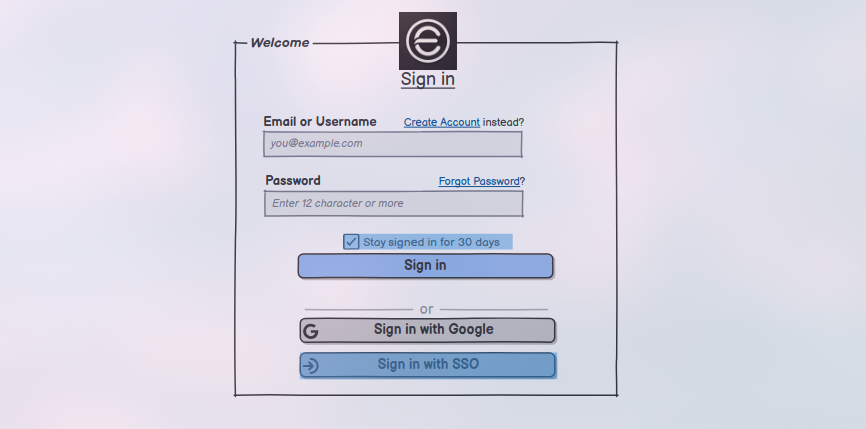
\includegraphics[width=1\textwidth]{Abbildungen/events/login.png}
    \caption{Login}
    \label{fig:login}
  \end{figure}
\subsection{Events}
\subsubsection{Event-Feed}
\begin{figure}[H]
    \centering
    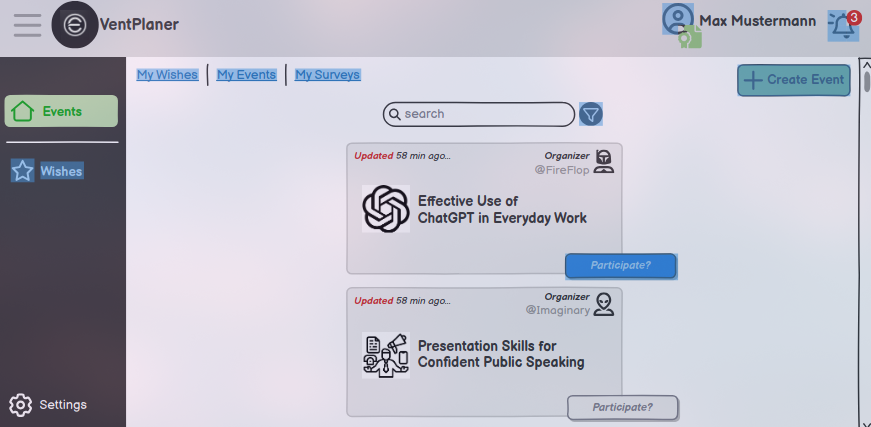
\includegraphics[width=1\textwidth]{Abbildungen/events/event_feed.png}
    \caption{Event-Feed}
    \label{fig:event_Feed}
  \end{figure}
\subsubsection{My Events}
\begin{figure}[H]
    \centering
    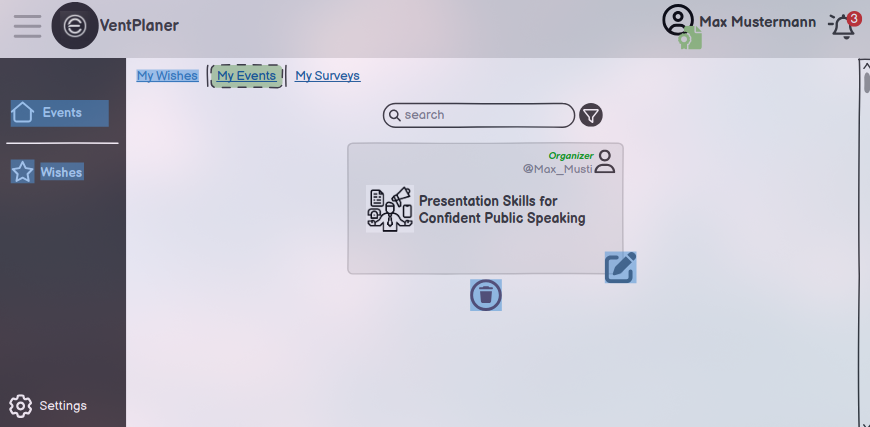
\includegraphics[width=1\textwidth]{Abbildungen/events/my_events.png}
    \caption{My Events}
    \label{fig:my_events}
  \end{figure}
\subsubsection{Event erstellen}
\begin{figure}[H]
    \centering
    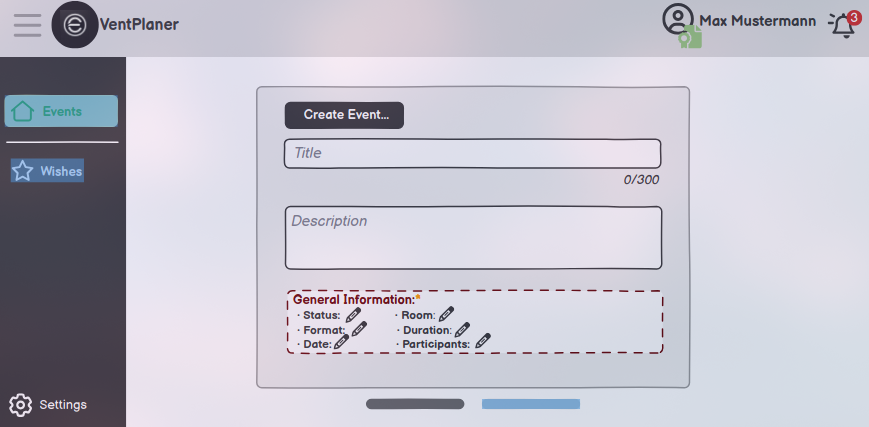
\includegraphics[width=1\textwidth]{Abbildungen/events/create_event.png}
    \caption{Event erstellen}
    \label{fig:create_event}
  \end{figure}
\subsubsection{Umfrage erstellen}
\begin{figure}[H]
    \centering
    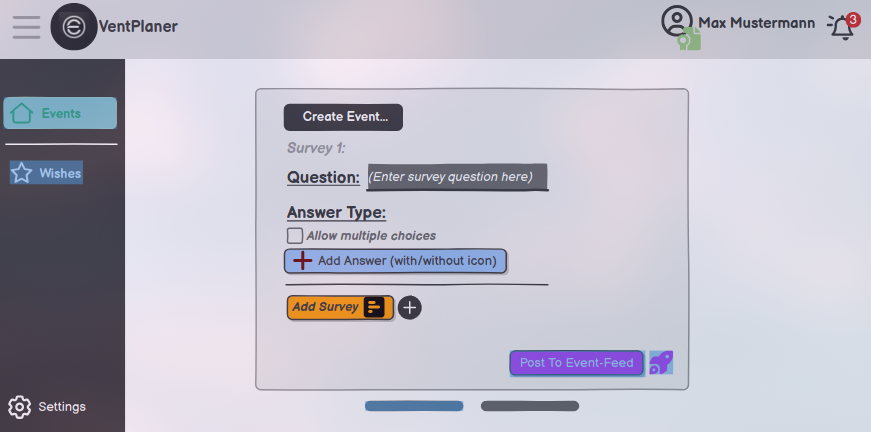
\includegraphics[width=1\textwidth]{Abbildungen/events/create_survey.png}
    \caption{Umfrage erstellen}
    \label{fig:create_survey}
  \end{figure}
\subsubsection{Umfrage bearbeiten}
\begin{figure}[H]
    \centering
    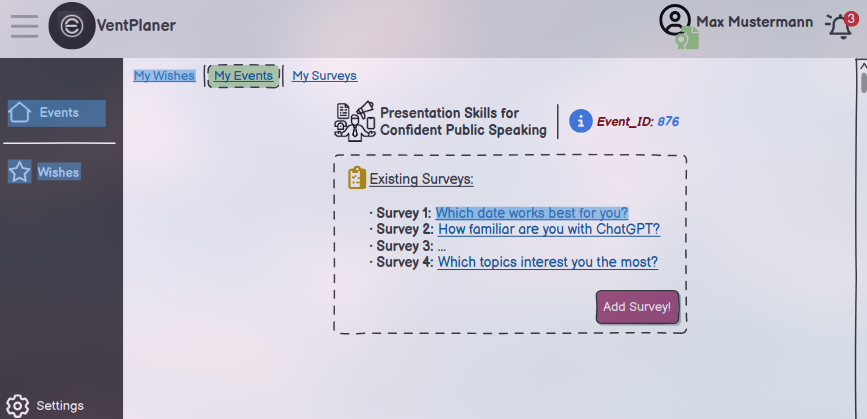
\includegraphics[width=1\textwidth]{Abbildungen/events/edit_survey.png}
    \caption{Umfrage bearbeiten}
    \label{fig:edit_survey}
  \end{figure}
\subsubsection{Meine Umfragen}
  \begin{figure}[H]
      \centering
      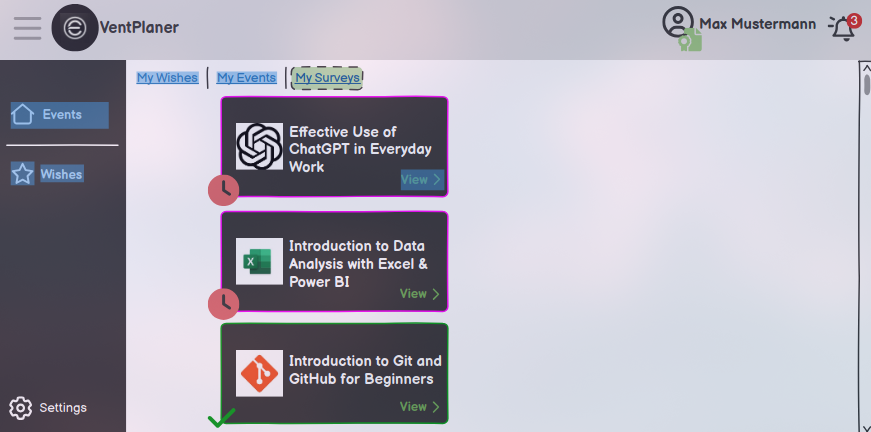
\includegraphics[width=1\textwidth]{Abbildungen/events/my_surveys.png}
      \caption{Meine Umfragen}
      \label{fig:my_survey}
    \end{figure}
\subsubsection{Event bearbeiten}
\begin{figure}[H]
    \centering
    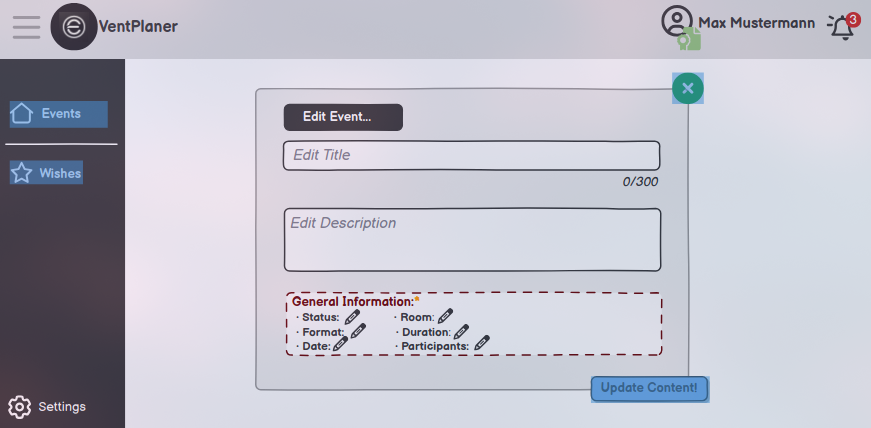
\includegraphics[width=1\textwidth]{Abbildungen/events/edit_event.png}
    \caption{Event bearbeiten}
    \label{fig:cedit_event}
  \end{figure}
\subsubsection{Event löschen}
\begin{figure}[H]
    \centering
    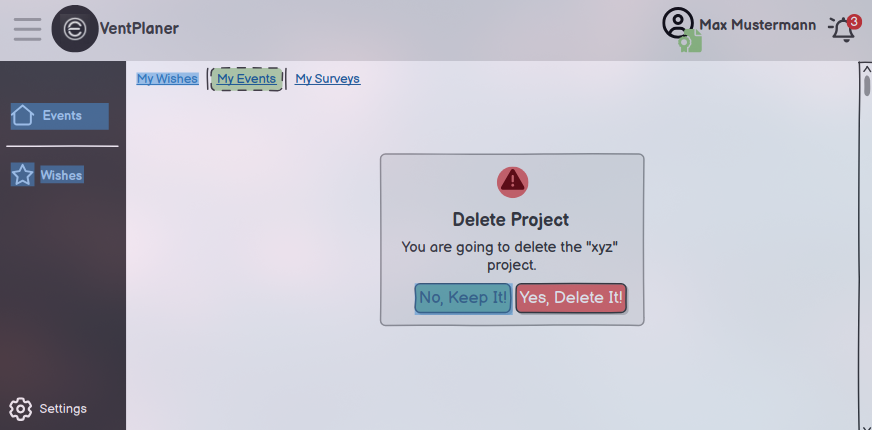
\includegraphics[width=1\textwidth]{Abbildungen/events/delete_event.png}
    \caption{Event löschen}
    \label{fig:delet_event}
  \end{figure}
\subsection{Wünsche}
\subsubsection{Wünsche-Feed}
\begin{figure}[H]
    \centering
    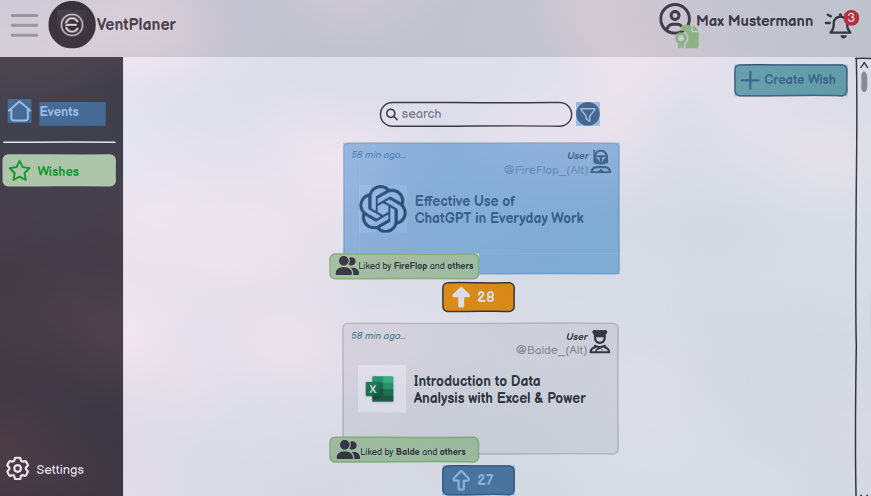
\includegraphics[width=1\textwidth]{Abbildungen/wishes/wishes-feed.png}
    \caption{Wünsche-Feed}
    \label{fig:wishes-feed}
  \end{figure}
\subsubsection{Meine Wünsche}
\begin{figure}[H]
    \centering
    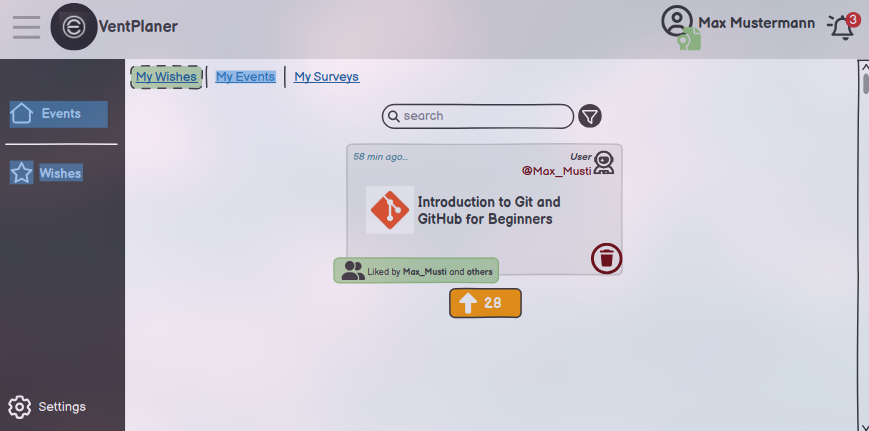
\includegraphics[width=1\textwidth]{Abbildungen/wishes/my-wishes.png}
    \caption{Meine Wünsche}
    \label{fig:my-wishes}
  \end{figure}
\subsubsection{Wunsch erstellen}
\begin{figure}[H]
    \centering
    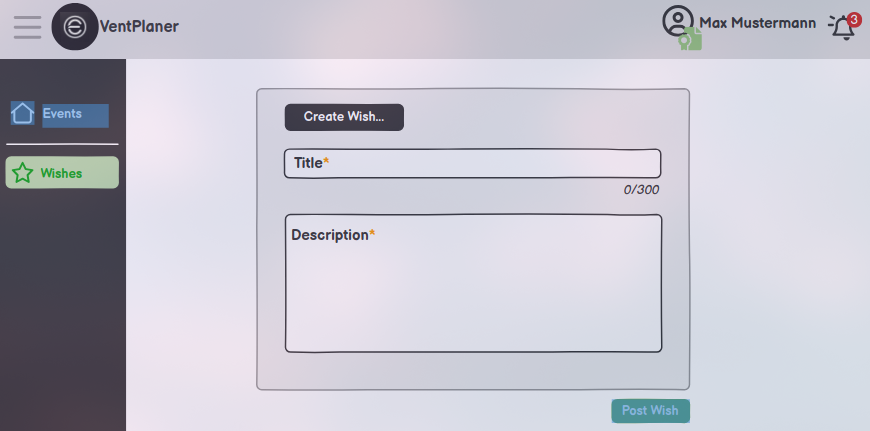
\includegraphics[width=1\textwidth]{Abbildungen/wishes/create_wish.png}
    \caption{Wunsch erstellen}
    \label{fig:create_wish}
  \end{figure}
\newpage
\section{Aufwandsschätzung}
\subsection{Anforderungsanalyse}
In dieser Phase werden die Anforderungen des Event-Planer festgelegt, einschließlich der Features und Funktionalitäten
\begin{itemize}
    \item Dauer: 1 Woche
\end{itemize}
\subsection{Entwurfsphase}
Es wird das Design bzw. die Struktur der Anwendung erstellt, einschließlich der Benutzeroberfläche, der Datenbankstruktur und der Systemarchitektur.
\begin{itemize}
    \item Dauer: 1-2 Woche
\end{itemize}
\subsection{Implementierung \& Testing}
Entwicklung der Anwendung basierend auf den festgelegten Anforderungen und dem Design bzw. der Struktur. Applikation soll direkt nach jedem Feature auf Funktion getestet werden
\begin{itemize}
    \item Dauer: 10 Wochen
    \begin{itemize}
        \item Einarbeitung Technologien: 2 Wochen
        \item Implementierung \& Testing: 8 Wochen
    \end{itemize}
\end{itemize}
\subsection{Bereitstellung und Projektabschluss}
Bereitstellung der Anwendung nach erfolgreicher Implementierung \& Testphase.
\begin{itemize}
    \item Dauer: 1-2 Wochen
\end{itemize}
\newpage
\section{Projektmanagement: A la Scrum}
Für dieses Projekt werden gewisse Apekte der agilen Methode Scrum verwendet. Dabei werden die Scrum-Zyklen auch bekannt als Sprints in 1 Wochen abschnitten eingeteilt, die sich durch schrittweise Entwicklung und durch regelmäßige Feedbackschleifen auszeichnet. Alle Aufgaben eines Sprints werden in Jira in einem Backlog gespeichert, beschrieben und unter dem Team verteilt.
\newline
\newline
Das Team hat wöchentliche Meetings mit dem Kunden und danach mit dem Betreuer des Projektes auch bekannt als Spint-Review. Dieser Termin findet immer Montags statt und markiert das Ende des aktuellen Sprints. Dieser Termin wird genutzt um die Ergebnisse des Kundes vom Sprint zu präsentieren und Feedback einzuholen, danach werden die nächsten Anforderungen vom Kunden besprochen. Im Anschluss darauf findet das Treffen mit dem Betreuer statt, bei denen offene fachliche Fragen geklärt werden. 
\newline
\newline
Die Sprints beginnen immer am Dienstag nachdem alle Anforderungen und Feedbacks eingesammelt worden sind. Des weiteren wurde der Sonntag als teaminternen Tag gekennzeichnet, bei dem weitere Fragen und Vorgehensweisen besprochen werden. Zudem werden die bearbeiteten Aufgaben durchgegangen und geklärt, was mit dem Kunden am Folgetag gesprochen wird. Nach dem Kundentreffen ist ein teaminternes Meeting angesetzt, bei welchem reflektiert wird, wie der letzte Sprint lief und mögliche Verbesserungen angesprochen werden. 
\newline
\newline
Im Ablauf der Sprints werden 2 Daily Standup-Meetings inkludiert, da mehrere Dailys im Rahmen dieses Projekts unrealistisch sind. Allerdings sind die Teammitglieder die ganze Woche erreichbar, um Unterstützung zu leisten und spontane Treffen einzurichten. Als Kommunikationsmittel wird teamintern ein Discord-Channel verwendet und für die Betreuer- sowie Kundentreffen hingegen Microsoft-Team.
\newpage
\section{Systemarchitektur}
Die Architektur des Gesamtsystems ist in einer Full-Stack Komponente unterteilt, auch bekannt als 2-Tier-Architecture, da bei Next.js das Front- und Backend innerhalt eines Projektes liegen. Die einzige logische Trennung die man hat ist die zwischen der Applikation und der Datenbank. Die Datenbank und der Authentifizierungsservice erfolgt über Supabase und einem Provider im Falle des Projektes über Microsoft, dass auch SSO unterstützt.
\begin{figure}[h]
  \centering
  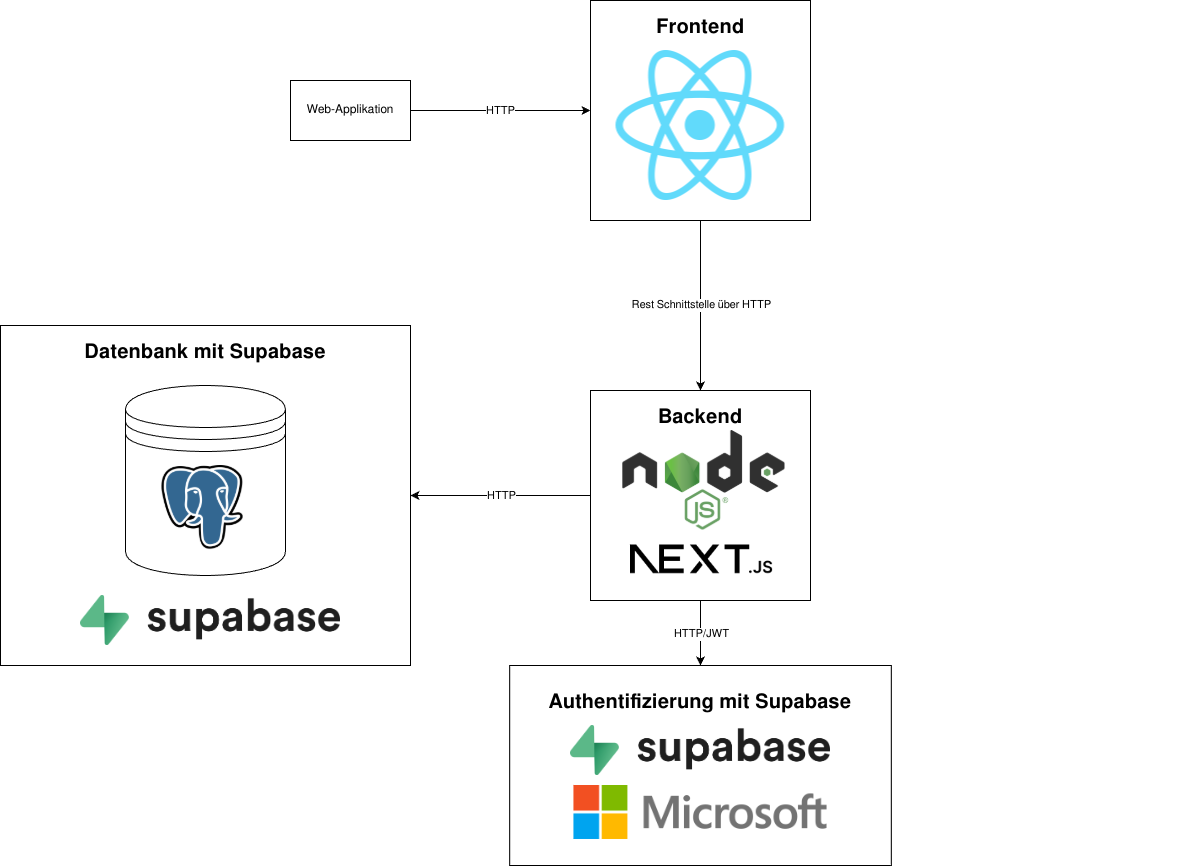
\includegraphics[width=1\textwidth]{Abbildungen/Systemarchitektur.png}
  \caption{Systemarchitektur}
  \label{fig:systemarchitektur}
\end{figure}
\newpage
\section{Literaturverzeichnis}
\end{document}
